\documentclass[12pt,letterpaper,titlepage,en-US]{article}

\usepackage{basicstyle}
\usepackage{homework}
%
% Homework Details
%   - Title
%   - Due date
%   - Class
%   - Section/Time
%   - Instructor
%   - Author
%

\newcommand{\hmwkTitle}{Homework\ \#4 }
\DTMsavetimestamp{DueDate}{2016-11-28T23:59:59-06:00}
\newcommand{\hmwkClass}{CS 6363.005}
\newcommand{\hmwkClassName}{Design and Analysis of Computer Algorithms}
\newcommand{\hmwkClassInstructor}{Instructor: Benjamin Raichel}
\newcommand{\hmwkAuthorName}{Hanlin He}
\newcommand{\hmwkAuthorNetID}{hxh160630}
\newcommand{\hmwkAuthorUTDEmail}{\href{mailto:hanlin.he@utdallas.edu}{hanlin.he@utdallas.edu}}


%
% Title Page
%

\title{
    \vspace{2in}
    \textmd{\textbf{\hmwkClassName \\\hmwkClass:\ \hmwkTitle}}\\
    \normalsize\vspace{0.1in}\small{Due\ on\ \DTMusedate{DueDate}\ at \DTMusetime{DueDate} }\\
    \vspace{0.1in}\large{\textit{\hmwkClassInstructor}}
    \vspace{3in}
}

\author{\textbf{\hmwkAuthorName\ \footnotesize{(\hmwkAuthorNetID)}} \\  \hmwkAuthorUTDEmail}
\date{}
\makeindex

\begin{document}
\maketitle

\pagenumbering{Roman}

\tableofcontents

\pagebreak
\pagenumbering{arabic}


\begin{homeworkProblem}[Running the Algorithms]
    \begin{homeworkSubProblem}[Dijkstra's Algorithm]
\begin{table}[H]
    \centering
    \begin{tabular}{c||ccccccl}
        Active &\ Null\ &\ s\ &\ a\ &\ d\ &\ b\ &\ c\ &\ e \tiny{(Final)}\\\hline\hline
        s & $0$ & & & & & & 0\\\hline
        a & $\infty$ & 3 & & & & & 3\\\hline
        b & $\infty$ & & 7 & & & & 7\\\hline
        c & $\infty$ & & 12 & 10 & 9 & & 9\\\hline
        d & $\infty$ & 6 & 5 & & & & 5\\\hline
        e & $\infty$ & & & 12 & 11 & 10 & 10\\
    \end{tabular}
\end{table}
\end{homeworkSubProblem}

\begin{homeworkSubProblem}[Bellman-Ford Algorithm]
Start from the edge with the smallest weight up to the edge with the largest weight.
The ordering is as follow:
\begin{enumerate}
    \item $c \rightarrow e$;
    \item $a \rightarrow d$ and $b \rightarrow c$;
    \item $s \rightarrow a$;
    \item $a \rightarrow b$.
\end{enumerate}
\end{homeworkSubProblem}
\end{homeworkProblem}

\begin{homeworkProblem}[SSSP]
Given a directed graph $G = (V,E)$, with positive edge weights and a single source shortest tree from vertex $s$.

Based on definition, for every vertex $v \in V$,
\begin{itemize}
    \item $dist(v) = pred(v) + w(pred(v) \rightarrow v)$;
    \item if $v \rightarrow w \in E$,
        then $dist(w) \leq dist(v) + w(v \rightarrow w)$.
\end{itemize}

Otherwise, the SSSP tree is wrong.

Thus, we can traverse the graph, at each vertex, check these values to verify the correctness.
The algorithm is shown in \cref{checksssp} applying DFS.

\begin{algorithm}[H]
    \caption{Algorithm to Check Correctness of SSSP}\label{checksssp}
    \begin{algorithmic}[1]
        \Procedure{CheckSSSP}{$v$}
            \State Mark $v$
            \For{each edge $v \rightarrow w$}
                \If{$dist(v) \neq pred(v) + w(pred(v) \rightarrow v)$}
                    \Return \textsc{False}
                \EndIf
                \If{$dist(w) > dist(v) + w(v \rightarrow w)$}
                    \Return \textsc{False}
                \ElsIf{$dist(w) = dist(v) + w(v \rightarrow w)$}
                    \If{$dist(w) \neq v$}
                        \Return \textsc{False}
                    \EndIf
                \EndIf
                \If{$w$ is unmarked.}
                    \Return\ProcedureName{CheckSSSP}{w}
                \EndIf
            \EndFor
        \EndProcedure
    \end{algorithmic}
\end{algorithm}

\end{homeworkProblem}

\begin{homeworkProblem}[Computing Flows and Cuts]
    \begin{homeworkSubProblem}[Residual Graph]

The residual graph of the flow network is shown in \cref{p3a}.
\begin{figure}[H]
    \caption{Residual Graph}\label{p3a}
    \centering
    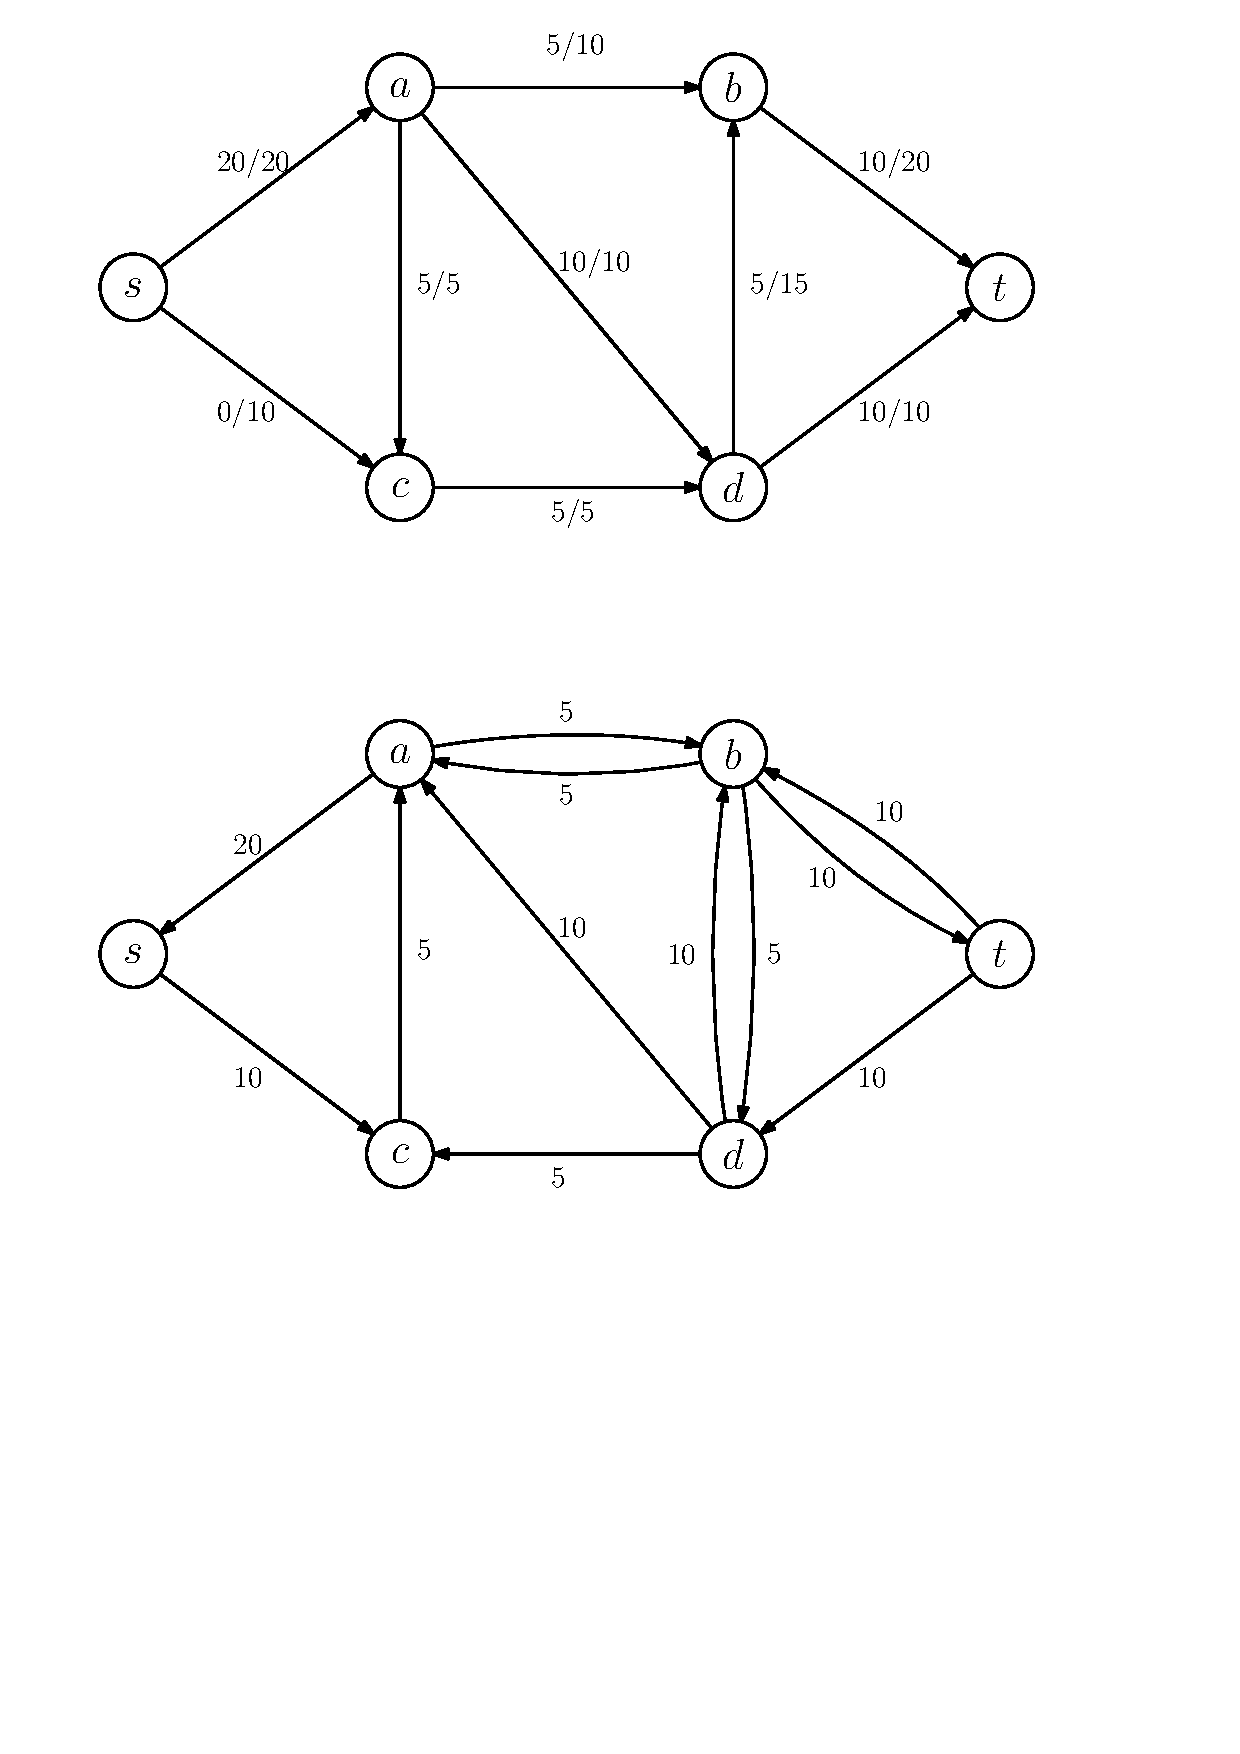
\includegraphics[width=.6\textwidth]{p3a}
\end{figure}


\end{homeworkSubProblem}
\begin{homeworkSubProblem}[Augmenting Path]
From the residual graph we know that,
\[s \longrightarrow c \longrightarrow a \longrightarrow b \longrightarrow t\]
is an augmenting path, as shown in \cref{p3b}.
\begin{figure}[H]
    \caption{Residual Graph}\label{p3b}
    \centering
    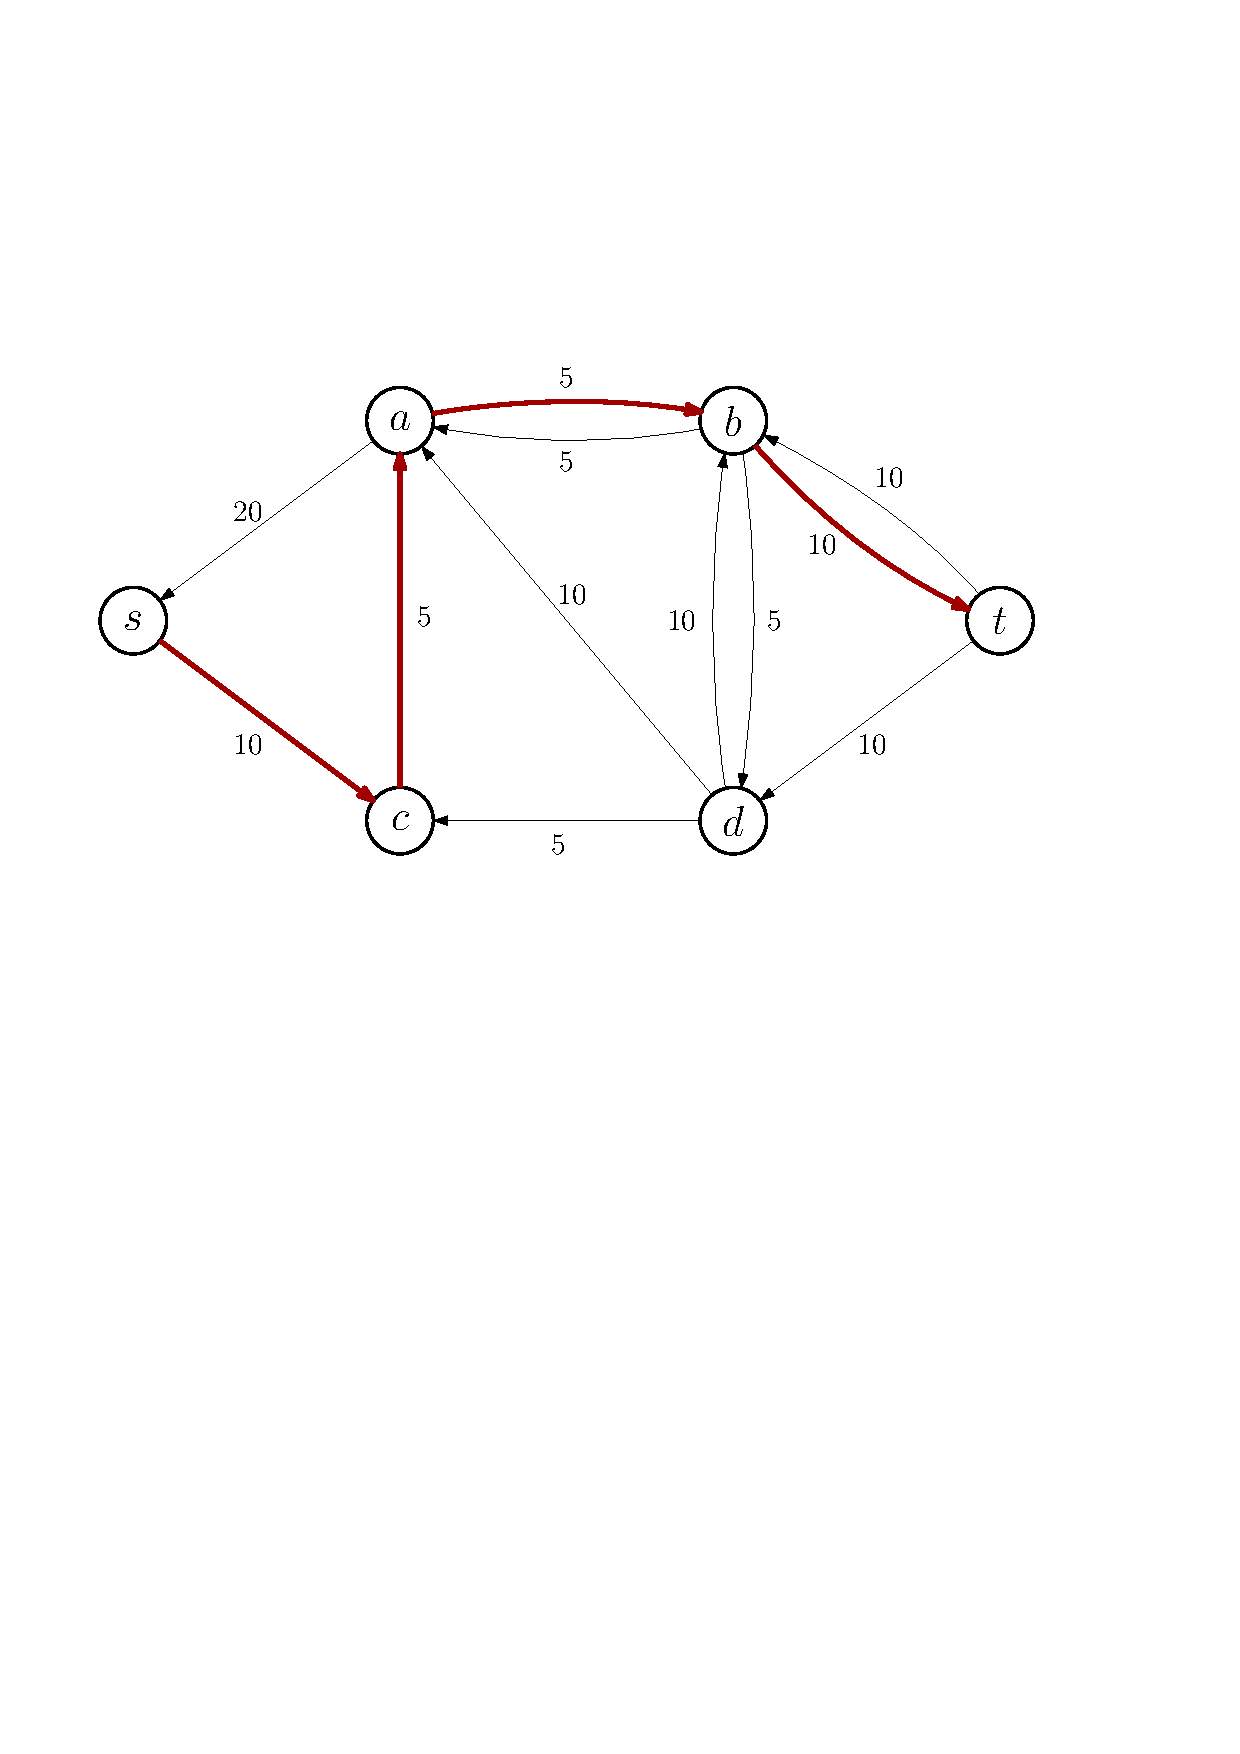
\includegraphics[width=.6\textwidth]{p3b}
\end{figure}

\begin{homeworkSubProblem}[Minimum Cut]
A minimum $s-t$ cut is $\{s,a,c\}$ and $\{b,d,t\}$, as shown in \cref{p3c}.
\begin{figure}[H]
    \caption{Residual Graph}\label{p3c}
    \centering
    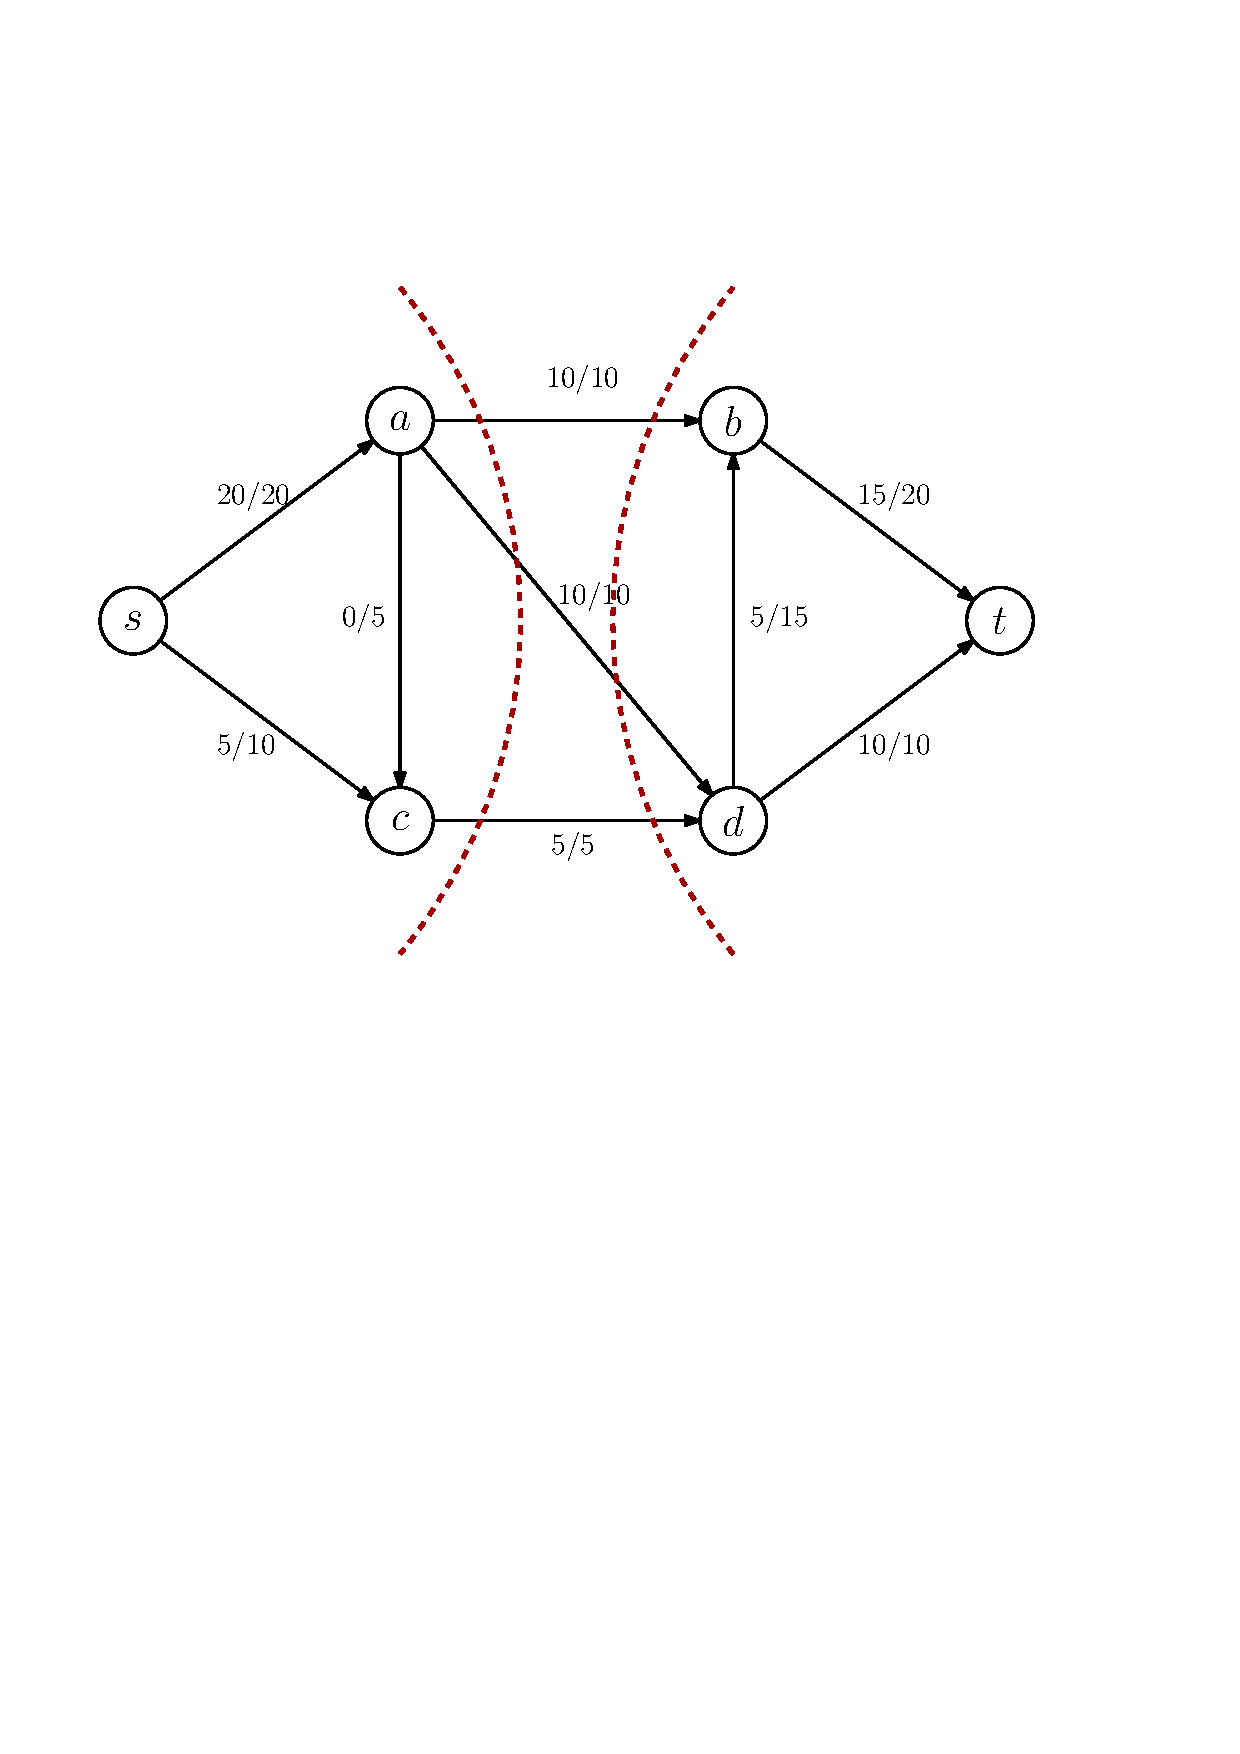
\includegraphics[width=.6\textwidth]{p3c}
\end{figure}
\end{homeworkSubProblem}
\end{homeworkSubProblem}
\end{homeworkProblem}

\begin{homeworkProblem}[Flow and Cut Problems]
    \begin{homeworkSubProblem}[Class Scheduling]
First, let $S$, the set of student, be the source of the graph.
Turn each student's interest classes $C(x_i)$ into a node,
and turn each class $C_i$ into a node.
Let $T$ denote the target, the sum of the enrolled total in each class.

Then,
\begin{enumerate}[label={(\arabic*)},leftmargin=.5in]
    \item Add a directed edge from $S$ to each $C(x_i)$ with capacity of $5$,
        representing a student can choose at most $5$ classes.
    \item Add a directed edge from each $C(x_i)$ to each $C_i$ contained in $C(x_I)$ with capacity of $1$,
        representing a student can register for specific class in the interest list at most once.
    \item Add a directed edge from each $C_i$ to $T$ with capacity of $20$,
        representing a class can have at most 20 enrolled students.
\end{enumerate}

Compute the maximum flow from $S$ to $T$ would be the maximum class enrollment.
The maximum flow graph is shown in \cref{p4a}.

\begin{figure}[H]
    \caption{Example}\label{p4a}
    \centering
    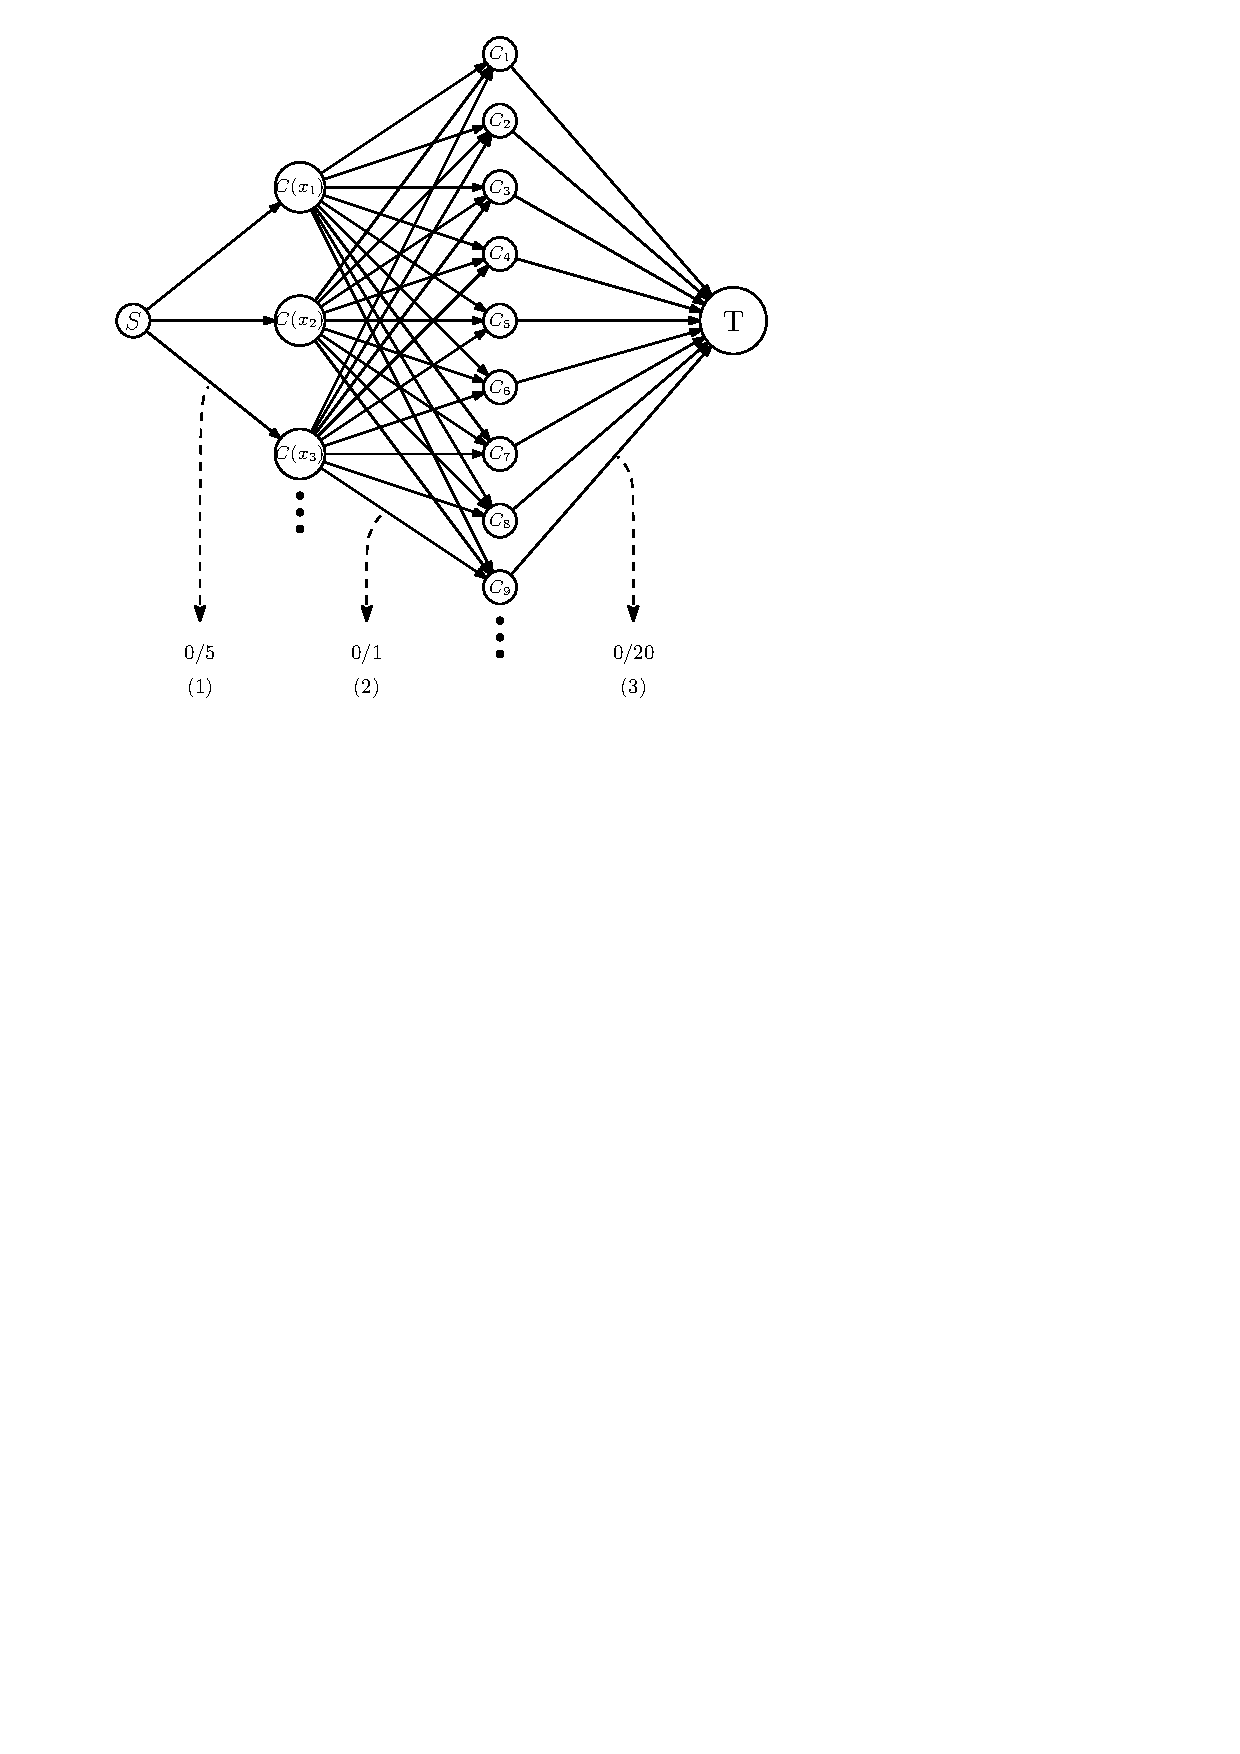
\includegraphics[width=.6\textwidth]{p4a}
\end{figure}


\end{homeworkSubProblem}
\begin{homeworkSubProblem}[Double Target Flow]
Add a third target node in $G$, with two directed edges of infinite capacity from $t_1$ and $t_2$ to $t$,
meaning $c(t_1 \rightarrow t) = \infty$, $c(t_2 \rightarrow t) = \infty$.
Then, the double target flow network is turned into a single target flow network,
where $t$ is the target.

It is obvious that the valid flow that maximizing the net flow
leaving $s$ is the same in both graph.
Hence, we can solve the problem using a standard flow algorithm.

The graph is shown in \cref{p4b}.
\begin{figure}[H]
    \caption{Turn Double Target Flow Into Standard Flow}\label{p4b}
    \centering
    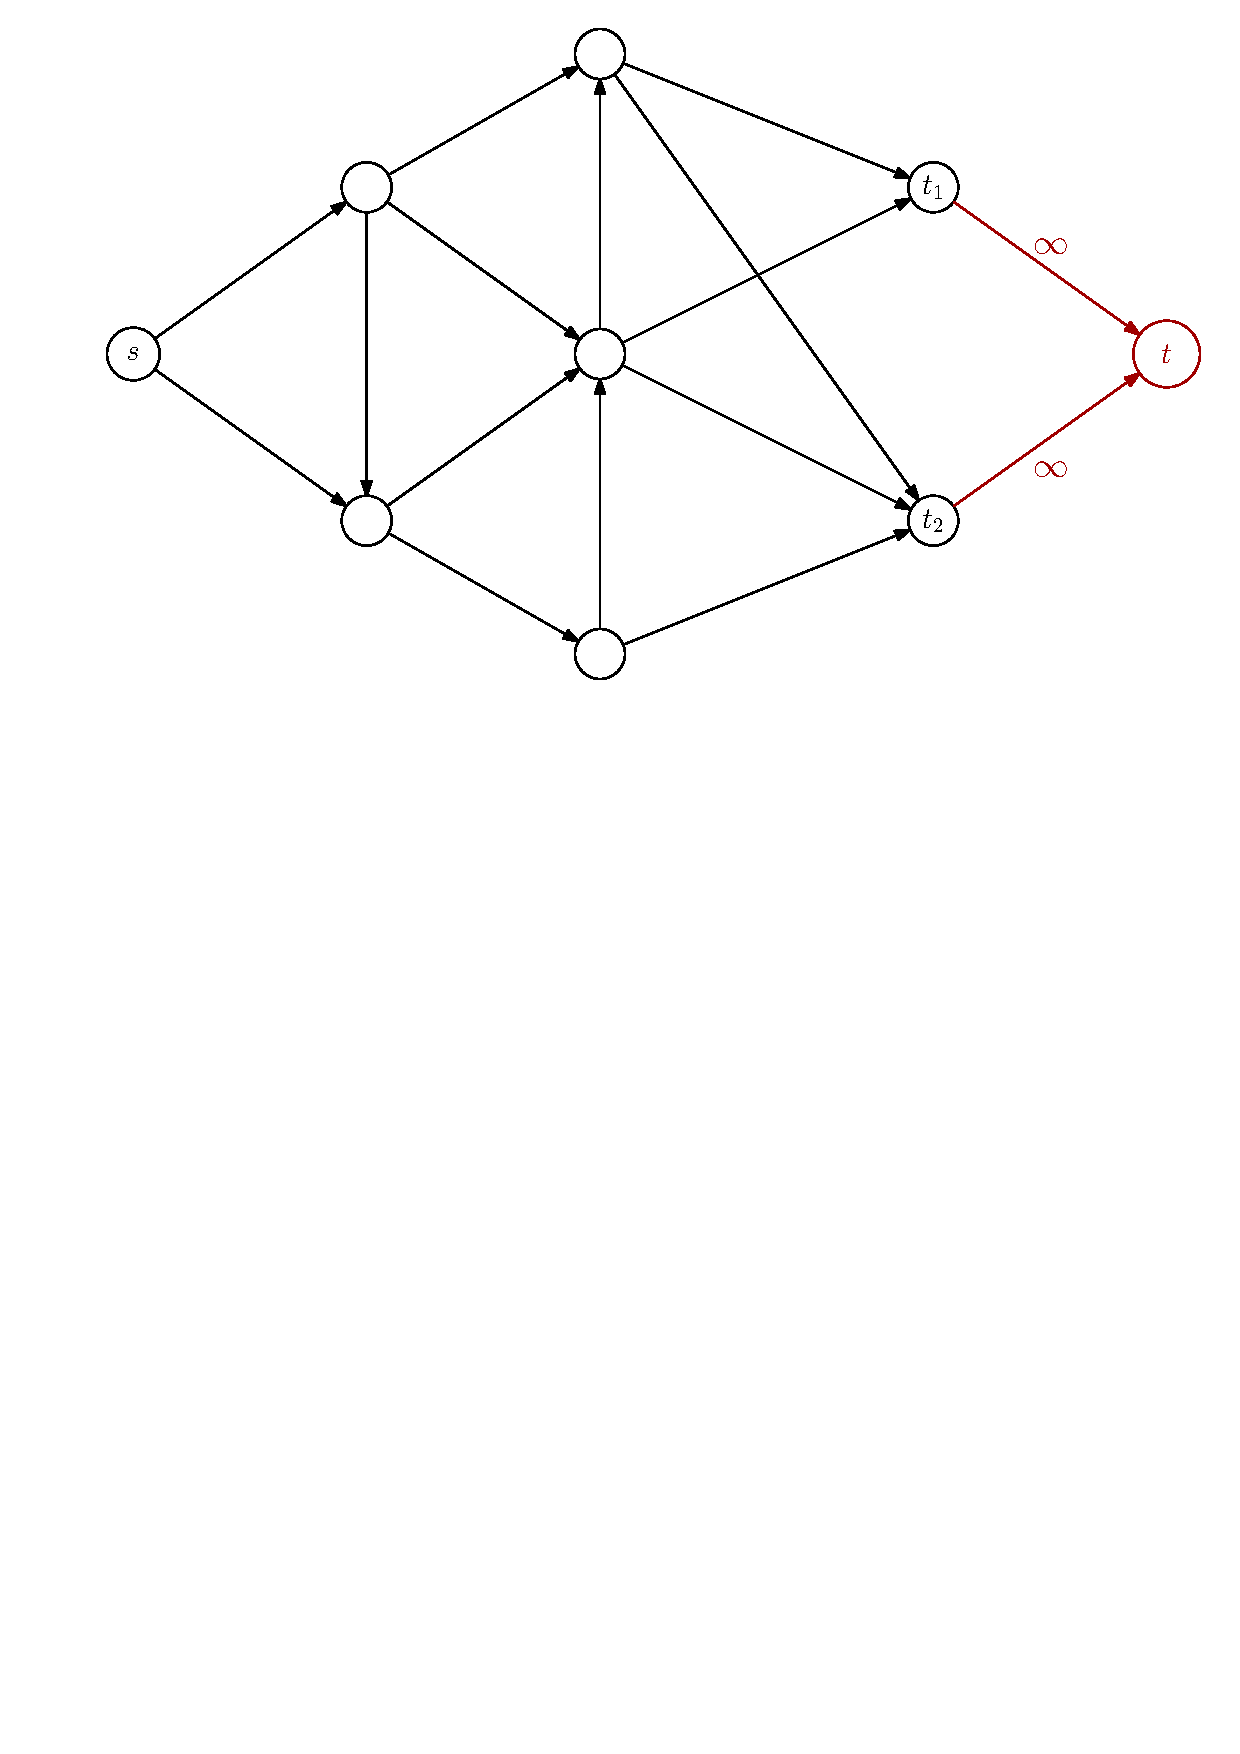
\includegraphics[width=.7\textwidth]{p4b}
\end{figure}

Let \ProcedureName{StandardMaxFlow}{G, s, t} be the given algorithm
to compute the max flow in any standard flow.
The algorithm is shown in \cref{double}.
\begin{algorithm}[H]
    \caption{Algorithm to Solve Double Target Maximum Flow}\label{double}
    \begin{algorithmic}[1]
        \Procedure{DoubleMaxFlow}{$G,s,t_1,t_2$}
            \State Add vertex $t$ to $G$, namely $G^\prime$. Add edges from $t_1,t_2$ to $t$ in $G^\prime$
            \State $c(t_1 \rightarrow t) = \infty$
            \State $c(t_2 \rightarrow t) = \infty$
            \Return \ProcedureName{StandardMaxFlow}{G^\prime, s, t}
        \EndProcedure
    \end{algorithmic}
\end{algorithm}
\end{homeworkSubProblem}
\pagebreak
\begin{homeworkSubProblem}[Unique Cuts]
    The steps of the algorithm can be described as follow, let $f^*$ be a maximum flow of $s-t$.
    \begin{enumerate}
        \item Compute the residual graph of $f^*$, denoted by $G_f = (V,E_f)$.
        \item Traverse $G_f$ from the source, we can find a set of vertices
            reachable from source. Let $S$ be that set.
        \item Let $T = V \setminus S$. Reverse all the edges in $E_f$ which has endpoint in $T$,
            i.e. for all $v \rightarrow w \in E_f$ that $v,w \in T$, replace the edge with $w \rightarrow v$.
            Let $G^\prime = (T,E_f^\prime)$ be the new graph.
        \item Traverse $T$, find the set of all the vertices which can be reached from $t$.
            Let $T^\prime$ be the set.
        \item If $S \cap T^\prime = V$, there is a unique minimum cut.
            Otherwise, there is no unique minimum cut in $G$.
    \end{enumerate}

    \vspace{0.1in}
    \noindent \textbf{Running Time Analysis}

    \begin{enumerate}
        \item Computing residual graph takes \bigO{|E|} time.
        \item Traversing $G_f$ to get $S$ takes \bigO{|V|} time.
        \item Reversing the edges in $G_f$ takes \bigO{|V|} time.
        \item Traversing $G^\prime$ to get $T^\prime$ takes \bigO{|E|} time.
    \end{enumerate}
    In total, the algorithm takes \bigO{|V|+|E|} time.

\end{homeworkSubProblem}
\end{homeworkProblem}

\begin{homeworkProblem}[NP-completeness]
    \begin{homeworkSubProblem}[Knapsack Problem]
    \bigO{nb} time does not imply P=NP, since $b$ is not polynomial in the length of the input
    to the problem.\footnote{Cited from Wikipedia:
    \href{https://en.wikipedia.org/wiki/Knapsack_problem}{Knapsack Problem}}
\end{homeworkSubProblem}

\begin{homeworkSubProblem}[Independent-Set]
Use the idea of binary search.

Let \ProcedureName{Independent-Set}{G,k} return \textsc{True} if exist
an independent set of size greater than $k$, otherwise return \textsc{False}.

Search the max value in $[0 \ldots k]$.
First try $k/2$, if \ProcedureName{Independent-Set}{G,k/2} = \textsc{True},
call \ProcedureName{Independent-Set}{G, (k + k/2)/2},
otherwise 
call \ProcedureName{Independent-Set}{G, (0 + k/2)/2},
and recursively continue.
Stop until \textsc{True} is returned,
or has made $\lceil\log k\rceil$ recursive calls.

\end{homeworkSubProblem}

\begin{homeworkSubProblem}[4SAT]
Reduce 3SAT to 4SAT:

Change every 3CNF formula into a 4CNF formula.
\[a \lor b \lor c \longrightarrow (a \lor b \lor c \lor x) \land (a \lor b \lor c \lor \overline{x})\]

For each 3CNF formula of $n$ size, there is at most $\binom{n}{3}$ types of clauses.
So this operation takes \bigO{n^3} time ( polynomial time ).

Thus, a 3SAT is reduced to a 4SAT problem, plus a polynomial time operation.

By definition, 3SAT is a NP-hard problem. Hence, we conclude 4SAT is NP-hard.
And because 4SAT is a special case of 3SAT, so it can be verified in polynomial time,
thus, it is also in NP.
Therefore, 4SAT is NP-complete.\hfill\qedsymbol
\end{homeworkSubProblem}

\begin{homeworkSubProblem}[Hitting-Set]
Reduce Vertex-Cover to Hitting-Set:

Given an undirected graph $G$ on $n$ nodes and $m$ edges and a parameter $k$.
We define:
\begin{itemize}
    \item $S$ to be the set of nodes in $G$;
    \item $S_i$ to be the set of the
        two endpoints of edges $e_i$, i.e. $S_i = \{u,v\}, \forall e \in E \text{, where } e = (u,v)$;
    \item Let the parameter $k$ be the same $k$ we are given.
\end{itemize}
Then $G$ has a vertex cover of size $k$ if and only if set $S$ has a hitting set
of size $k$ for $C = \{S_1, \ldots , S_m\}$, since a set of nodes in $G$ is a vertex cover $S^\prime$
if and only if it has an element in common with each of the edges,
i.e. $S^\prime \cap S_i \neq \emptyset$.

This reduction is in polynomial time because we only need to list the edges
of $G$, which takes \bigO{n+m} time.
Therefore, Hitting-Set is NP-hard.

On the other hand, given a ``Hitting Set'', it takes \bigO{n^2} to find
the intersection of two set with size $n$. For totally $m$ set, it is checkable in polynomial
time (\bigO{n^2m} in particular), i.e. Hitting-Set is in NP.

Hence, Hitting-Set is NP-complete.\hfill\qedsymbol
\end{homeworkSubProblem}

\end{homeworkProblem}
\end{document}
